\subsubsection{概要}

一番初めのモデルで,自己排他性をうまく取り入れることができなかったために,
2つ目のモデルでは初めから質点間の距離を一定に保つようなルールを取り入れておいて,
その上で各質点に斥力ポテンシャルを導入することで自己排他性を持たせつつ,
点をランダムに追加していくという方法で線分の成長を表現することとした。

この考えをさらに推し進めてみると,質点の位置を2次元のユークリッド空間における点ではなく,
各格子点同士の距離が等しくなるような格子における格子点とすれば,隣接する質点とは必ず等しい距離に
保つことができる。
また,同じ格子点を占めることのできる質点の数を1つに限定することによって,自己排他性も担保されていることから,
2つめのモデルで考慮したかった条件は常に満たされるという意味で,格子状の点を考えることには意味があるように思われる。

ここでは,4回対称性を持つ正方格子よりも,6回対称性をもつ三角格子の方が取りうる線素のパターンの数は多いということから,
三角格子上でひも状構造を作り,その成長をモデル化することを目的とする。

\subsubsection{三角格子の作成}

プログラム上で三角格子を自然に定義しようとするならば,扱いやすい正方格子をもとに,
それを変形したものとして三角格子を扱うのが良いだろう。
即ち,図\ref{fig:trilattice}のように,正方格子の隣接関係にプラスしてさらに二つの格子点と隣接関係にあり,
それが図の番号のように対応しているとみなすことである。このようにしておけば実際のデータ構造としては2次元の行列上に情報を保存しておきつつ,
各格子点の隣接関係を参照できるようにしておくことで,描画などの際には三角格子として表現することが可能となる。

\begin{figure}[H]
  \begin{center}
    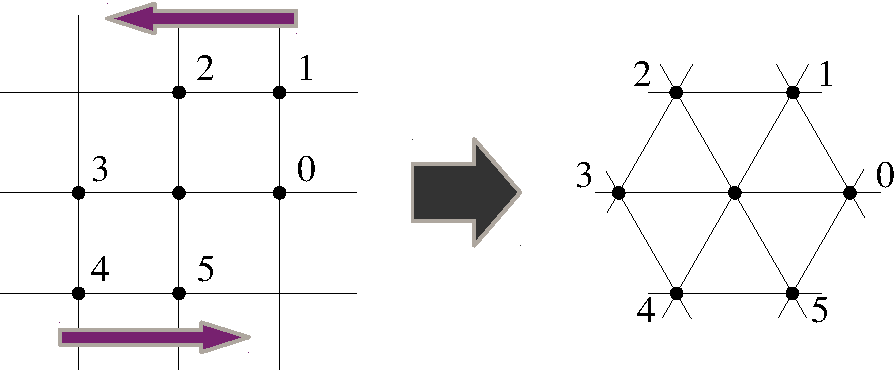
\includegraphics[width=0.7\textwidth]{../img/triangular_lattice.pdf}
    \caption{2次元正方格子を三角格子に対応させるための隣接関係の再定義}
    \label{fig:trilattice}
  \end{center}
\end{figure}

またこのとき,三角格子は周期境界条件を満たすようにする。

\subsubsection{三角格子状で定義されるひも状構造}

上のようにして作成された三角格子上で定義されるひも状オブジェクトの表し方を以下のように定める。

まず,始点(頭)となる格子点の座標(正方格子における(行, 列))を定める。
次に,始点から次の格子点へのベクトルを,図\ref{fig:unitvec}に示したような6方向の単位ベクトル
$\vector{u}_{\alpha}\ (\alpha \in \{0, 1, \dots , 5\})$のうちの一つで表現する。
同様に,2つ目の点に向かうベクトルを指定する。
このようなベクトルをオブジェクトの構成要素数だけつなげれば,全体を表すことができる。
また,この方法の利点は,格子を占有している点がどのひも状オブジェクトに属するものなのか,
ベクトルを遡ることで特定できるということである。

したがって,一つのひも状オブジェクト$S$は以下で決定される。
$$ S = ((x, y), (\alpha_{1},  \alpha_{2}, \dots , \alpha_{N-1}) ), \ \alpha_{i} \in \{0, 1, \dots , 5\}$$

\begin{figure}[H]
  \begin{center}
    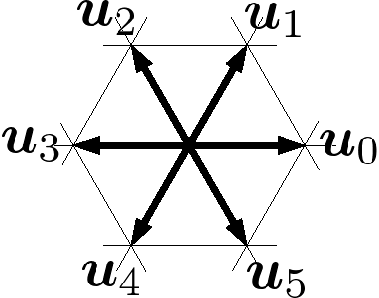
\includegraphics[width=0.5\textwidth]{../img/unitvec.pdf}
    \caption{6つの基本ベクトル}
    \label{fig:unitvec}
  \end{center}
\end{figure}

\subsubsection{ひも状構造の配置}

次に,ひも状構造を実際に三角格子の中に配置することを考える。
これは一見何でもないことのように思われるが,実際はオブジェクトの要素数が増大するにつれて,
重なりなく配置することは難しくなってくる.

これは,三角格子中の自己回避型ランダムウォーク(SAW)の問題として捉えることができる。

今は指定した個数の要素でオブジェクトが構成できればいいので,周囲の格子点がすべて占有されている状態(dealock状態と呼ぶ)となった時は,その一つ前の要素を配置する時点までさかのぼり,今回


